\chapter{Aplicações da Linguagem R}
  \begin{comment} //Cabeçalho
    Prof. Dr. Ausberto S. Castro Vera
    UENF - CCT - LCMAT - Curso de Ciência da Computação
    Campos, RJ,  2021
    Disciplina: Paradigmas de Linguagens de Programação
  \end{comment}
  \begin{comment} //Comentários iniciais
    Devem ser mostradas pelo menos CINCO aplicações completas da linguagem, e em cada caso deve ser apresentado:
    \begin{itemize}
      \item Uma breve descrição da aplicação,
      \item O código completo da aplicação,
      \item Imagens do código fonte no compilador-interpretador,
      \item Imagens dos resultados após a compilação-interpretação do código fonte
      \item Links e referências bibliográficas de onde foi obtido a aplicação
    \end{itemize}
  \end{comment}
  \section{Operações básicas}
  	\begin{itemize}
  		\item \textbf{Descrição}
  		
  		  O código abaixo mostrará os seguintes conceitos básicos presentes em linguagens de programação:
  		  \begin{enumerate}
  			\item Comentários
  			\item Imprimir informações
  			\item Fazer operações com variáveis
  			\item Obter dados pela entrada padrão
  			\item Operações Lógicas
  			\item Estruturas de controle de fluxo
  			\item Funções
  		\end{enumerate}
  		  Mais abaixo é mostrada a Figura \ref{Codigo_1} que apresenta a execução do código no ambiente de desenvolvimento RStudio.
  	
  		\item \textbf{Código}
  		\color{blue}
  		\verbatiminput{1-Operacoes_Basicas.r}
  		\color{black}
  		
  		  %\begin{lstlisting}[language=R]
  		  %\end{lstlisting}
  		  
  		\item \textbf{Imagens do código com resultados}
  		  \begin{figure}[H]  \label{Codigo_1}
  		  	\centering
  		  		\caption{Operações básicas no RStudio}
  		  		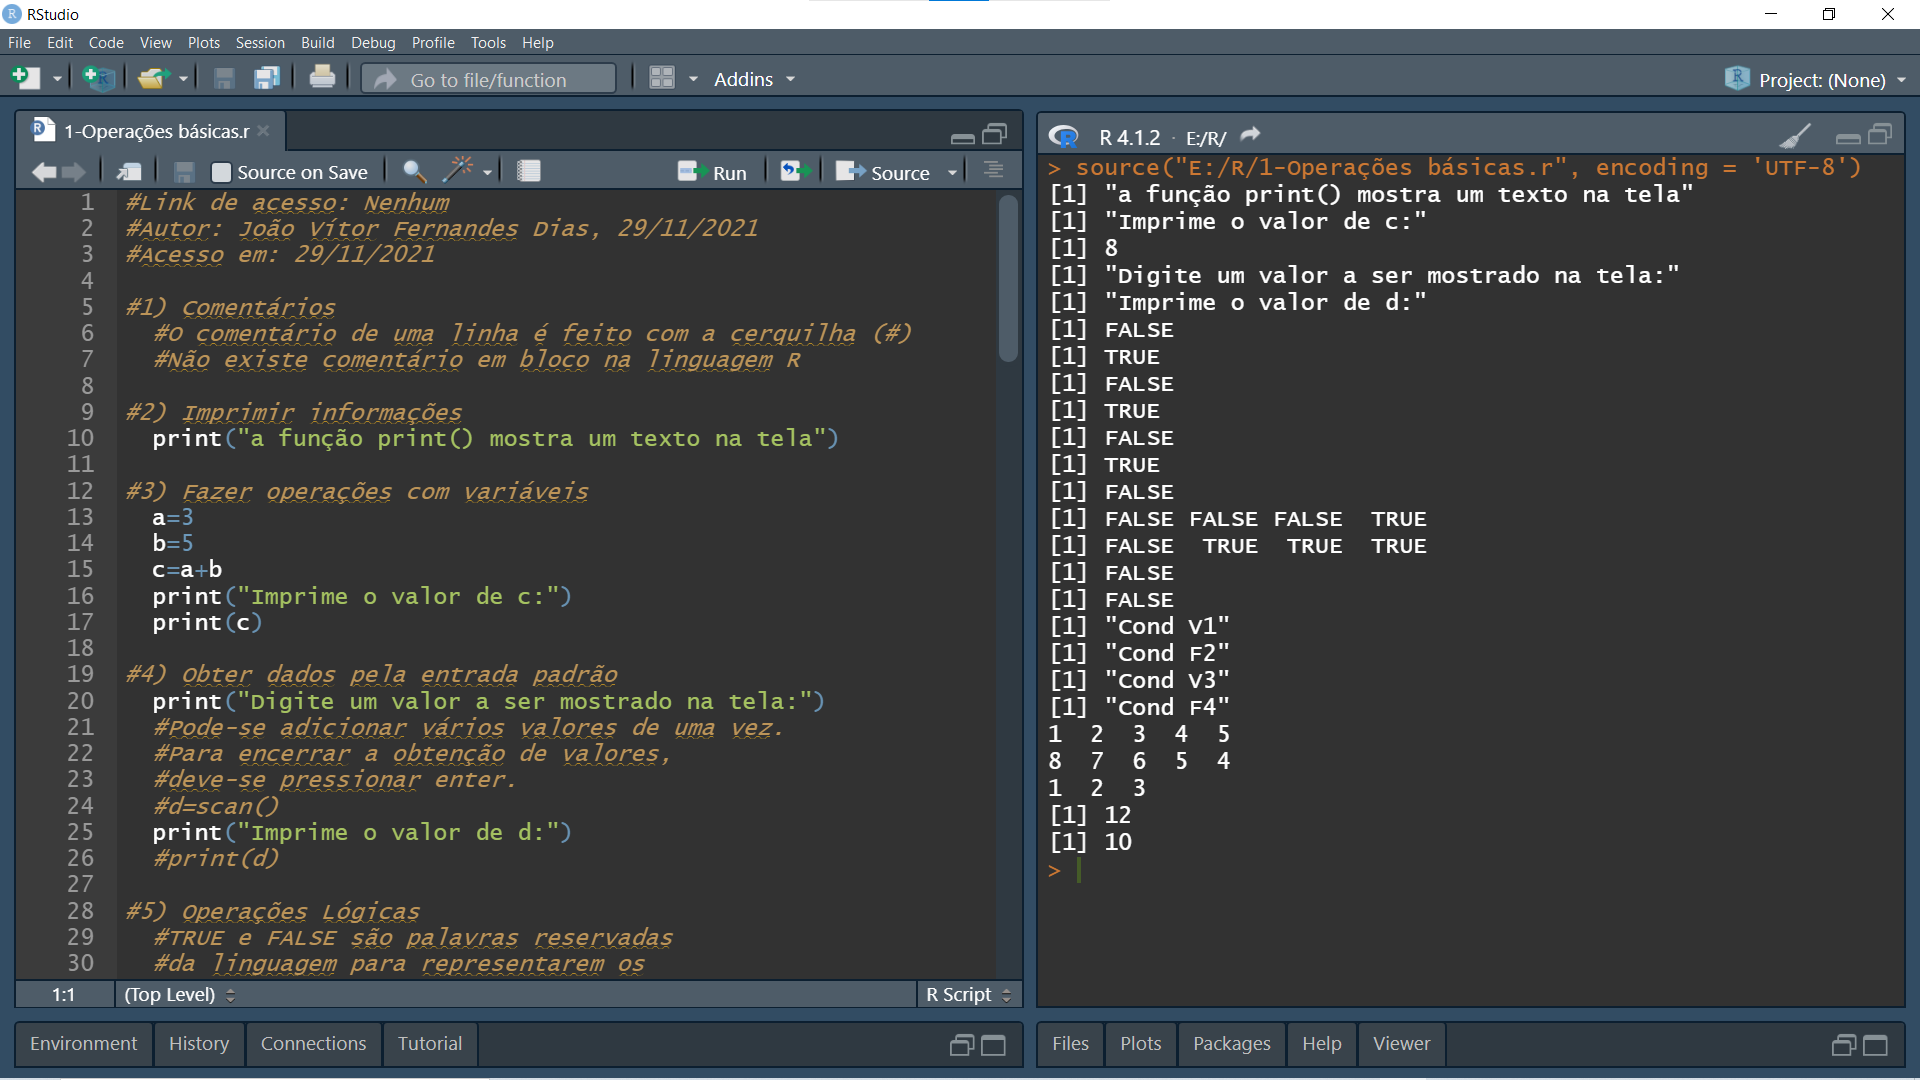
\includegraphics[width=16cm]{PicturesJoaoDias/Codigos/Codigo1.png}
  		  		{\tiny \sf Fonte: autoria própria}
  		  \end{figure}
  		  
  		\item \textbf{Links e referências bibliográficas das aplicações}
  		\\ \\
  		  Código de autoria própria.
  		
  	\end{itemize}
  
  \section{Programas gráficos}
  \begin{itemize}
  	\item \textbf{Descrição}
  	
  	  Este programa apresenta um código de exemplo para demonstrar a capacidade de diversidade de gráficos gerados em R. O exemplo escolhido apresenta um gráfico ternário representando as cores dos pixels de acordo com a quantidade de vermelho, verde e azul.
  	  
  	  Mais abaixo é mostrada a Figura \ref{Codigo_2a} que apresenta a execução do código no ambiente de desenvolvimento RStudio.
  	  %e também a Figura \ref{Codigo_2b} que apresenta o gráfico gerado pela execução do programa.
  	  
  	  
  	\item \textbf{Código}
  	
  	
  	\color{blue}
  	\verbatiminput{2-Programas_Graficos.r}
  	\color{black}
  	
  	\item \textbf{Imagens do código com resultados}
  	
	  	\begin{figure}[H]  \label{Codigo_2a}
	  		\centering
	  		\caption{Programas gráficos no RStudio}
	  		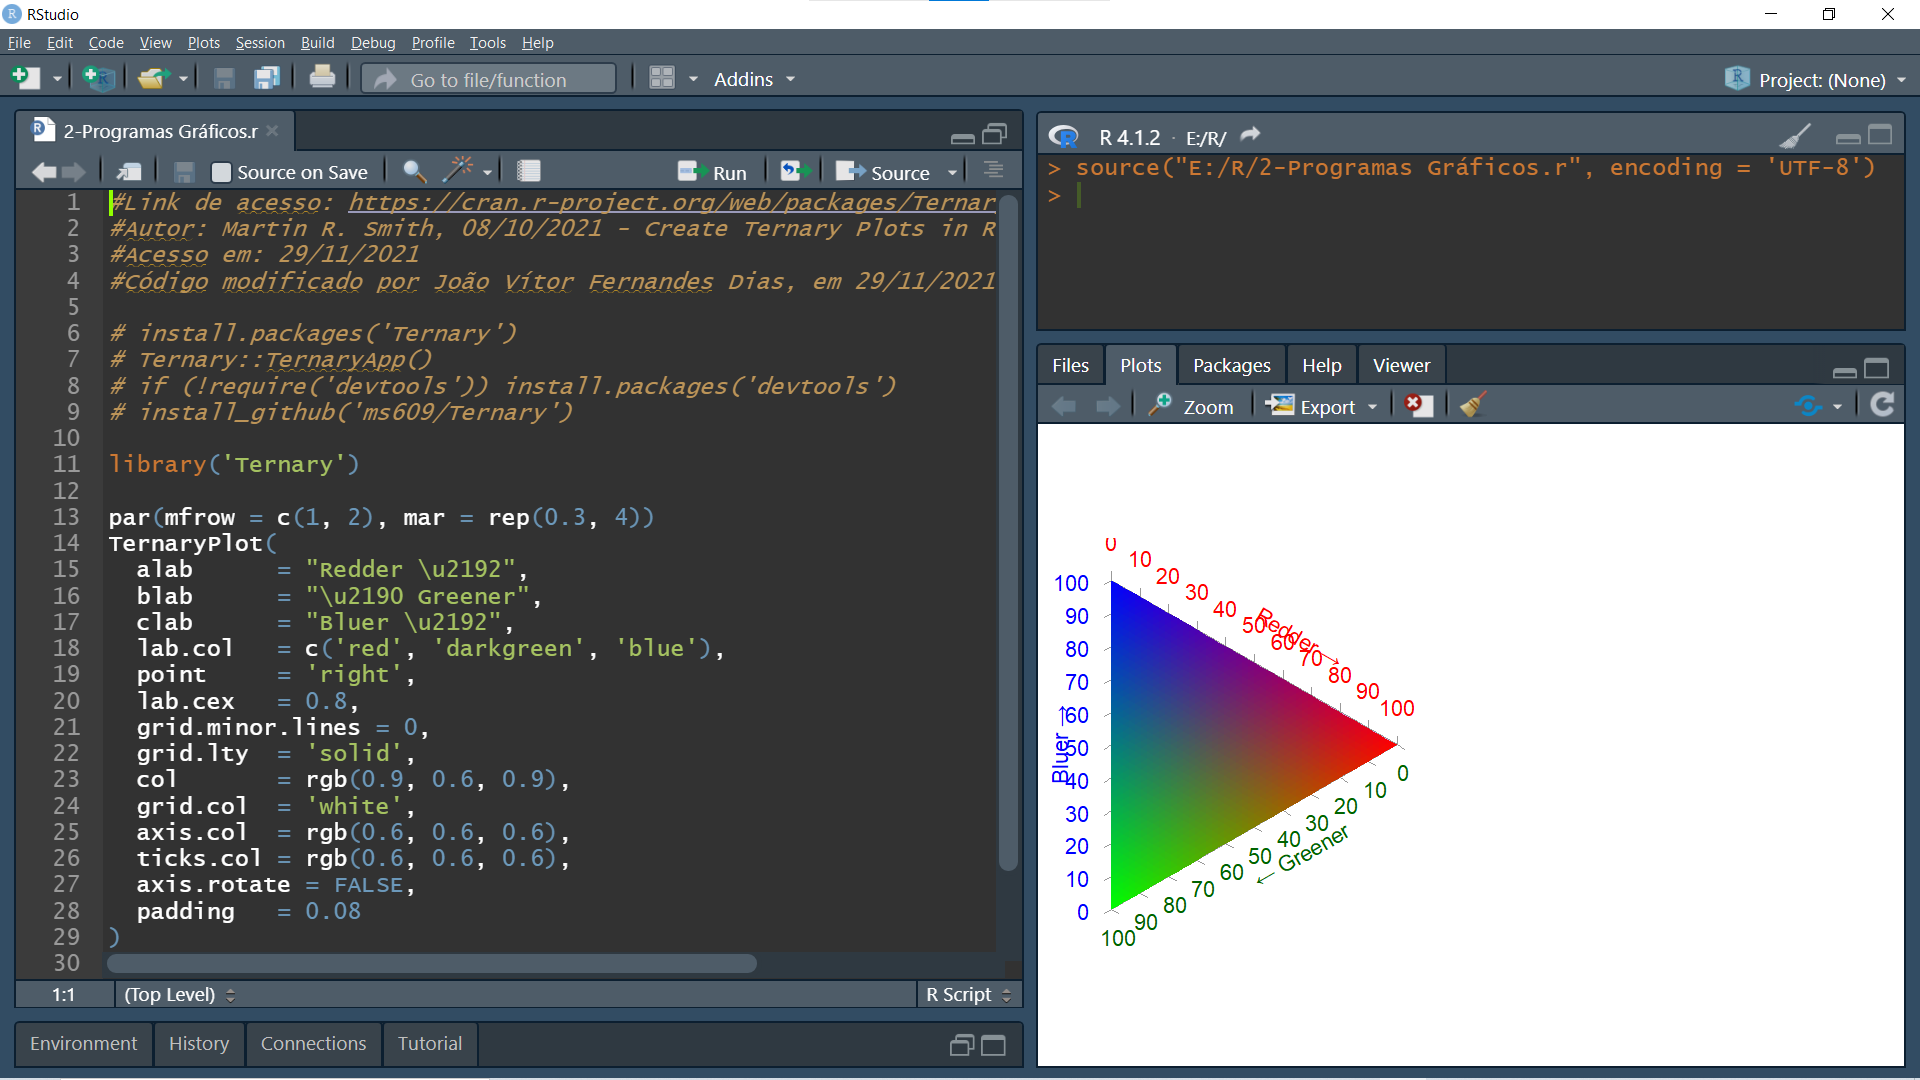
\includegraphics[width=16cm]{PicturesJoaoDias/Codigos/Codigo2a.png}
	  		{\tiny \sf Fonte: autoria própria}
	  	\end{figure}
	  	\begin{comment}	%IMAGEM SENDO REFERENCIADA DE FORMA ESTRANHA
	  		
	  	\begin{figure}[H]  \label{Codigo_2b}
	  		\centering
	  		\caption{Gráfico resultante}
	  		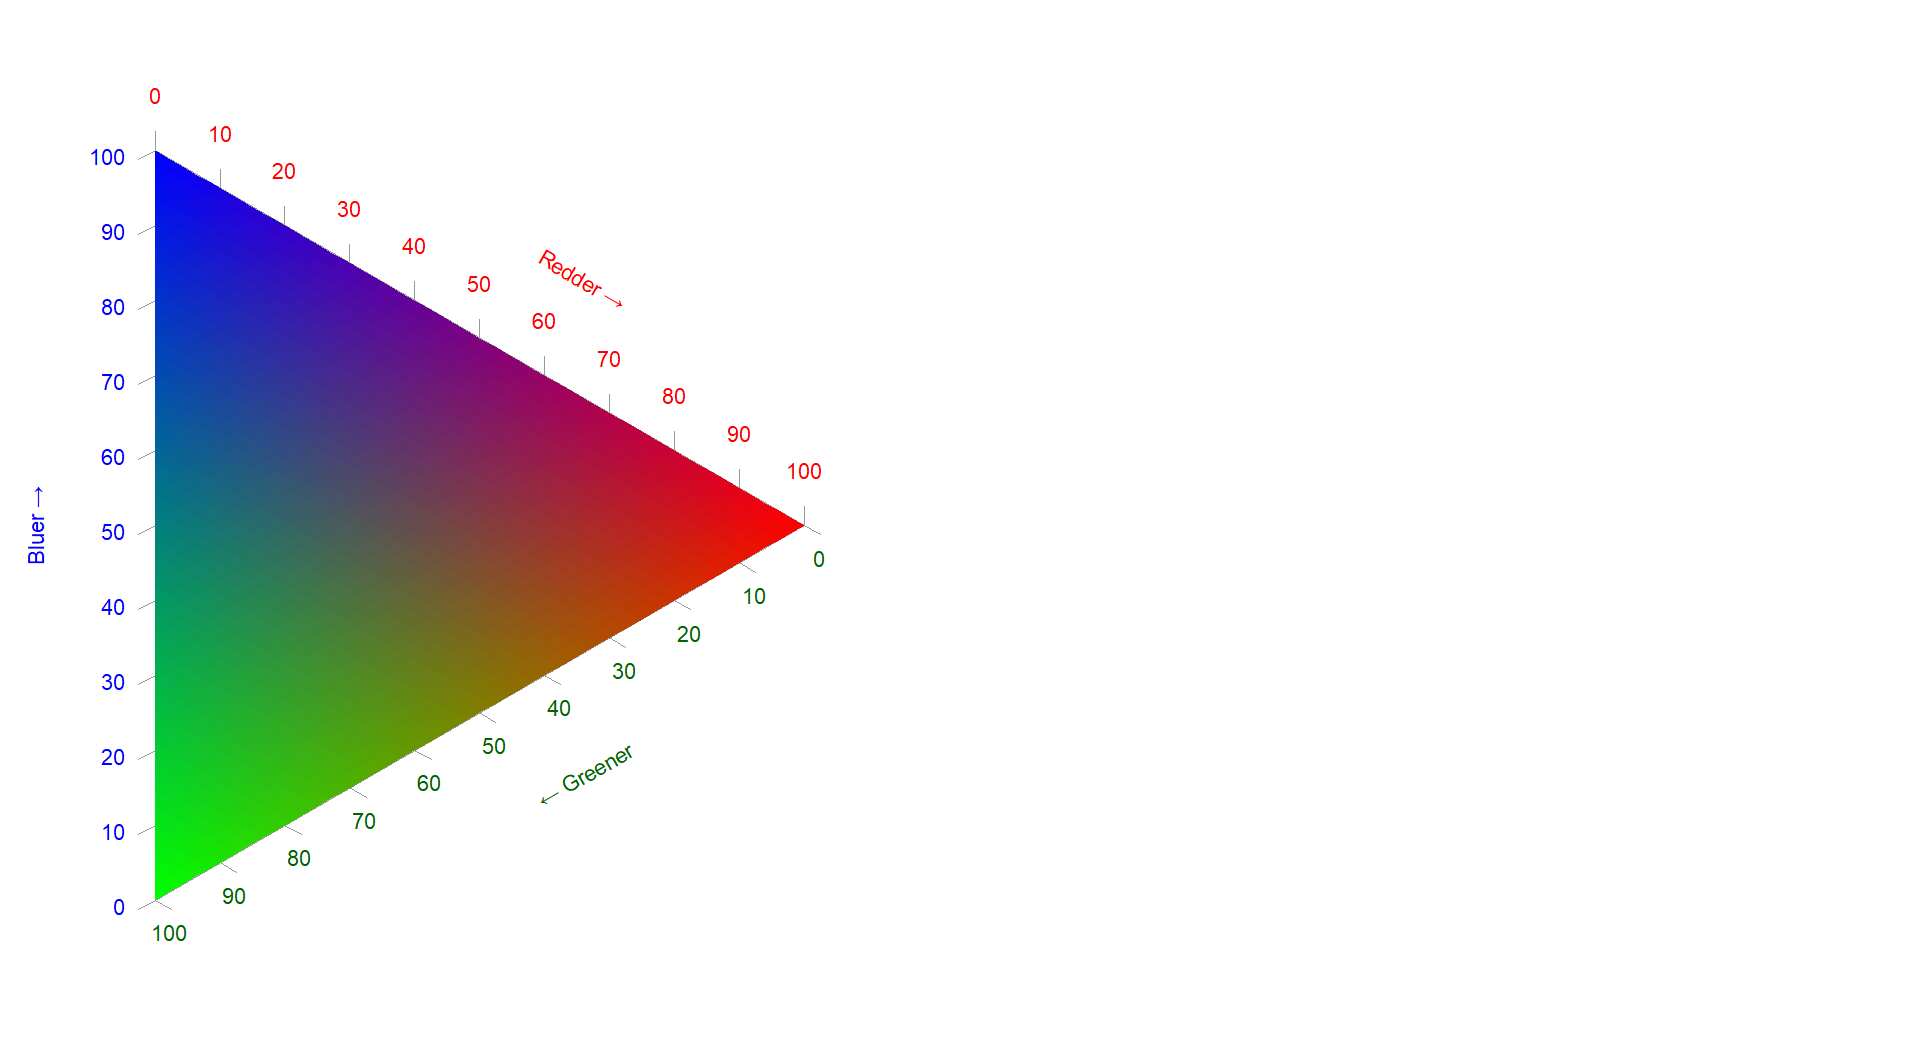
\includegraphics[width=16cm]{PicturesJoaoDias/Codigos/Codigo2b.png}
	  		{\tiny \sf Fonte: autoria própria}
	  	\end{figure}
  	
        \end{comment}
    
  	\item \textbf{Links e referências bibliográficas das aplicações}
  	  \\ \\
  	  \textit{Link referente ao código:} 
  	  \href{https://cran.r-project.org/web/packages/Ternary/vignettes/Ternary.html}{Create Ternary Plots in R}
  	
  	  \textit{Desenvolvido por:} Martin R. Smith, 08/10/2021
  	
  	  \textit{Acesso em:} 29/11/2021
  	
  \end{itemize}
  \section{Programas com Objetos}
  \begin{itemize}
  	\item \textbf{Descrição}
  	
  	  O código seguinte apresenta alguns exemplos de estruturas para criação de objetos e classes, utilizando a linguagem R. No código abaixo é criado um objeto endereço e também duas classes, uma classe S3 representando um cachorro, e uma classe S4 representando uma caneta.
  	  
  	  Mais abaixo é mostrada a Figura \ref{Codigo_3} que apresenta a execução do código no ambiente de desenvolvimento RStudio.
  	
  	\item \textbf{Código} 
  	
  	\color{blue}
  	\verbatiminput{3-Objetos.r}
  	\color{black}
  	
  	\item \textbf{Imagens do código com resultados}
	  	
	  	\begin{figure}[H]  \label{Codigo_3}
	  		\centering
	  		\caption{Programas com objetos no RStudio}
	  		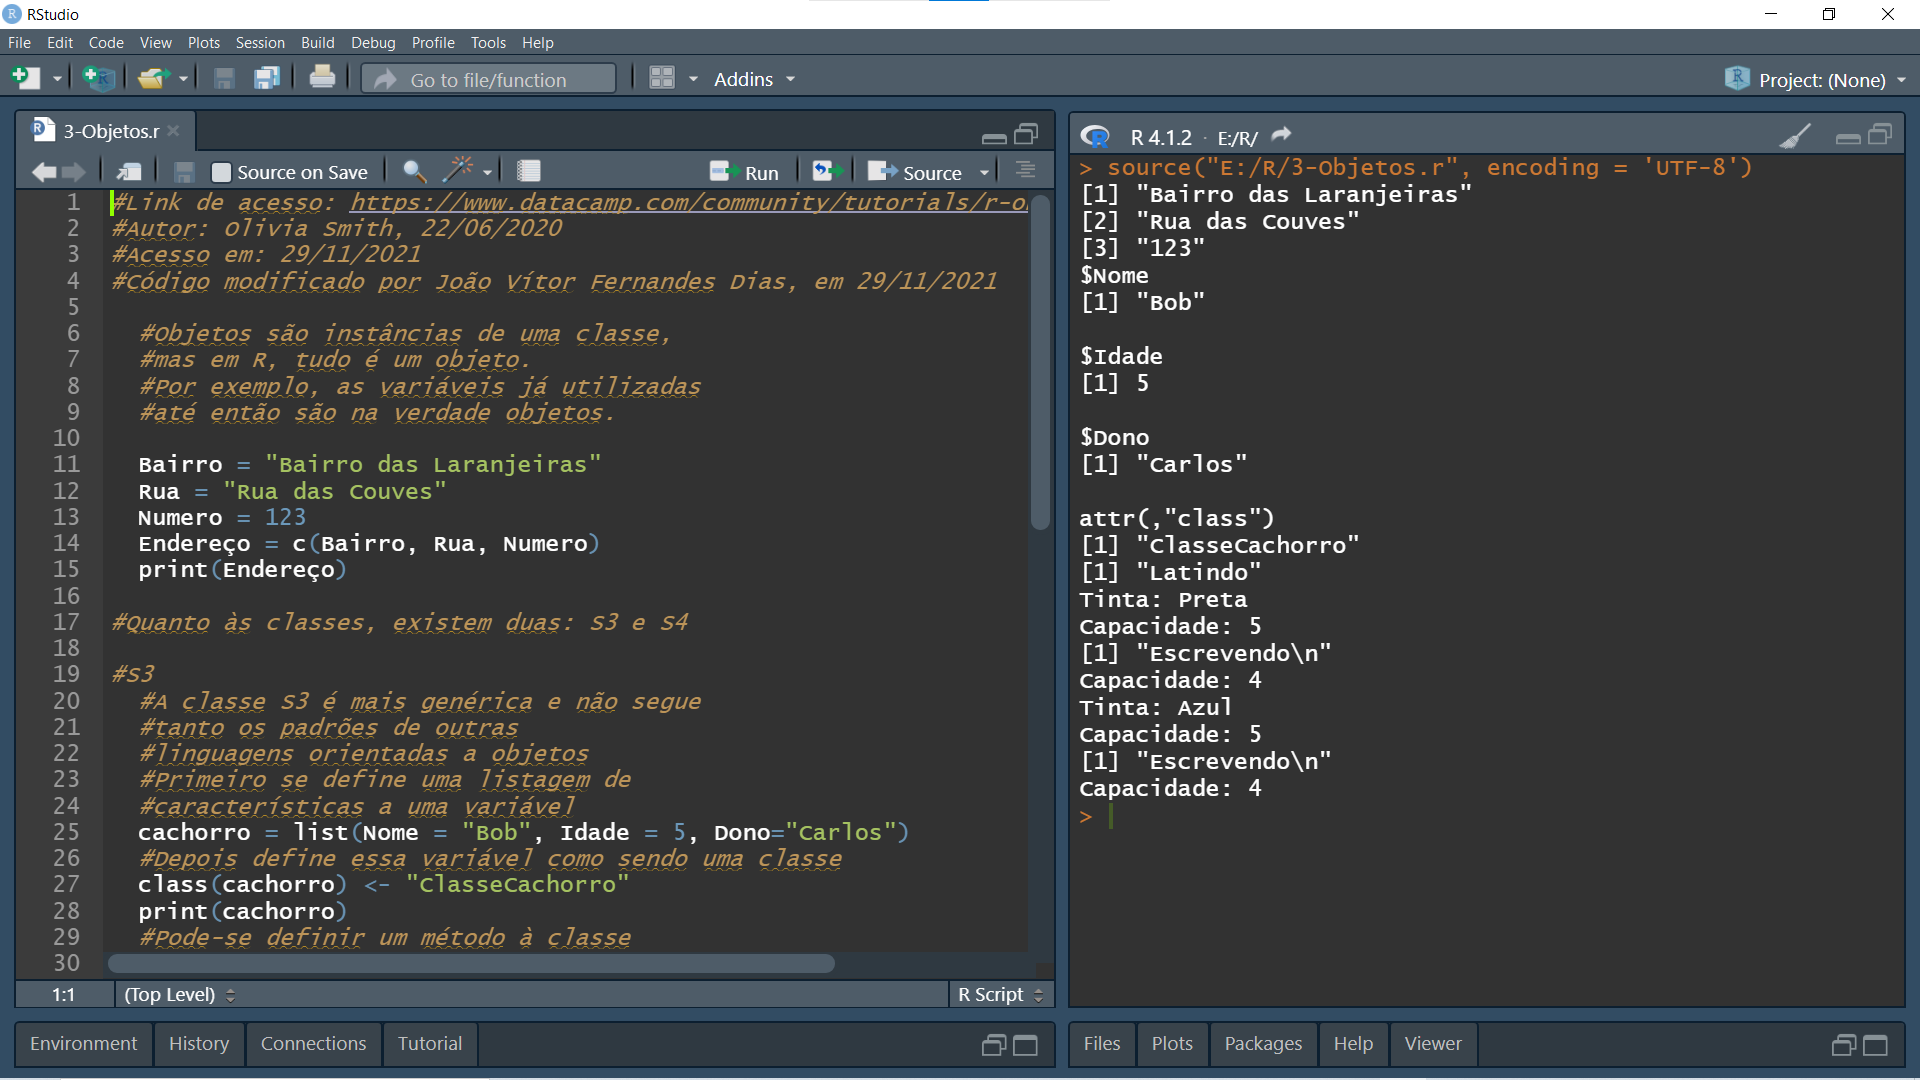
\includegraphics[width=16cm]{PicturesJoaoDias/Codigos/Codigo3.png}
	  		{\tiny \sf Fonte: autoria própria}
	  	\end{figure}
  	
  	\item \textbf{Links e referências bibliográficas das aplicações}
  	  \\ \\
  	  \textit{Link referente ao código:} 
  	  \href{https://www.datacamp.com/community/tutorials/r-objects-and-classes}{R objects and classes}
  	
  	  \textit{Desenvolvido por:} Olivia Smith, 22/06/2020
  	
  	  \textit{Acesso em:} 29/11/2021
  	
  \end{itemize}
	
  \section{O algoritmo Quicksort - Implementação}
  \begin{itemize}
  	\item \textbf{Descrição}
  	  
  	  O código abaixo apresenta uma forma recursiva do conhecido algoritmo de Quicksort, onde ele recursivamente seleciona um elemento pivô e separa o vetor entre elementos maiores e menores que ele, até que reste apenas um elemento a ser comparado, então retorna os valores e obtém-se o vetor ordenado.
  	
  	  Mais abaixo é mostrada a Figura \ref{Codigo_4} que representa a execução do código no ambiente de desenvolvimento RStudio Cloud.
  	
  	\item \textbf{Código}
  	
  	\color{blue}
  	\verbatiminput{4-QuickSort.r}
  	\color{black}
  	
  	\item \textbf{O algoritmo Quicksort no RStudio Cloud}
  	
      \begin{figure}[H]  \label{Codigo_4}
        \centering
        \caption{O algoritmo Quicksort no RStudio Cloud}
        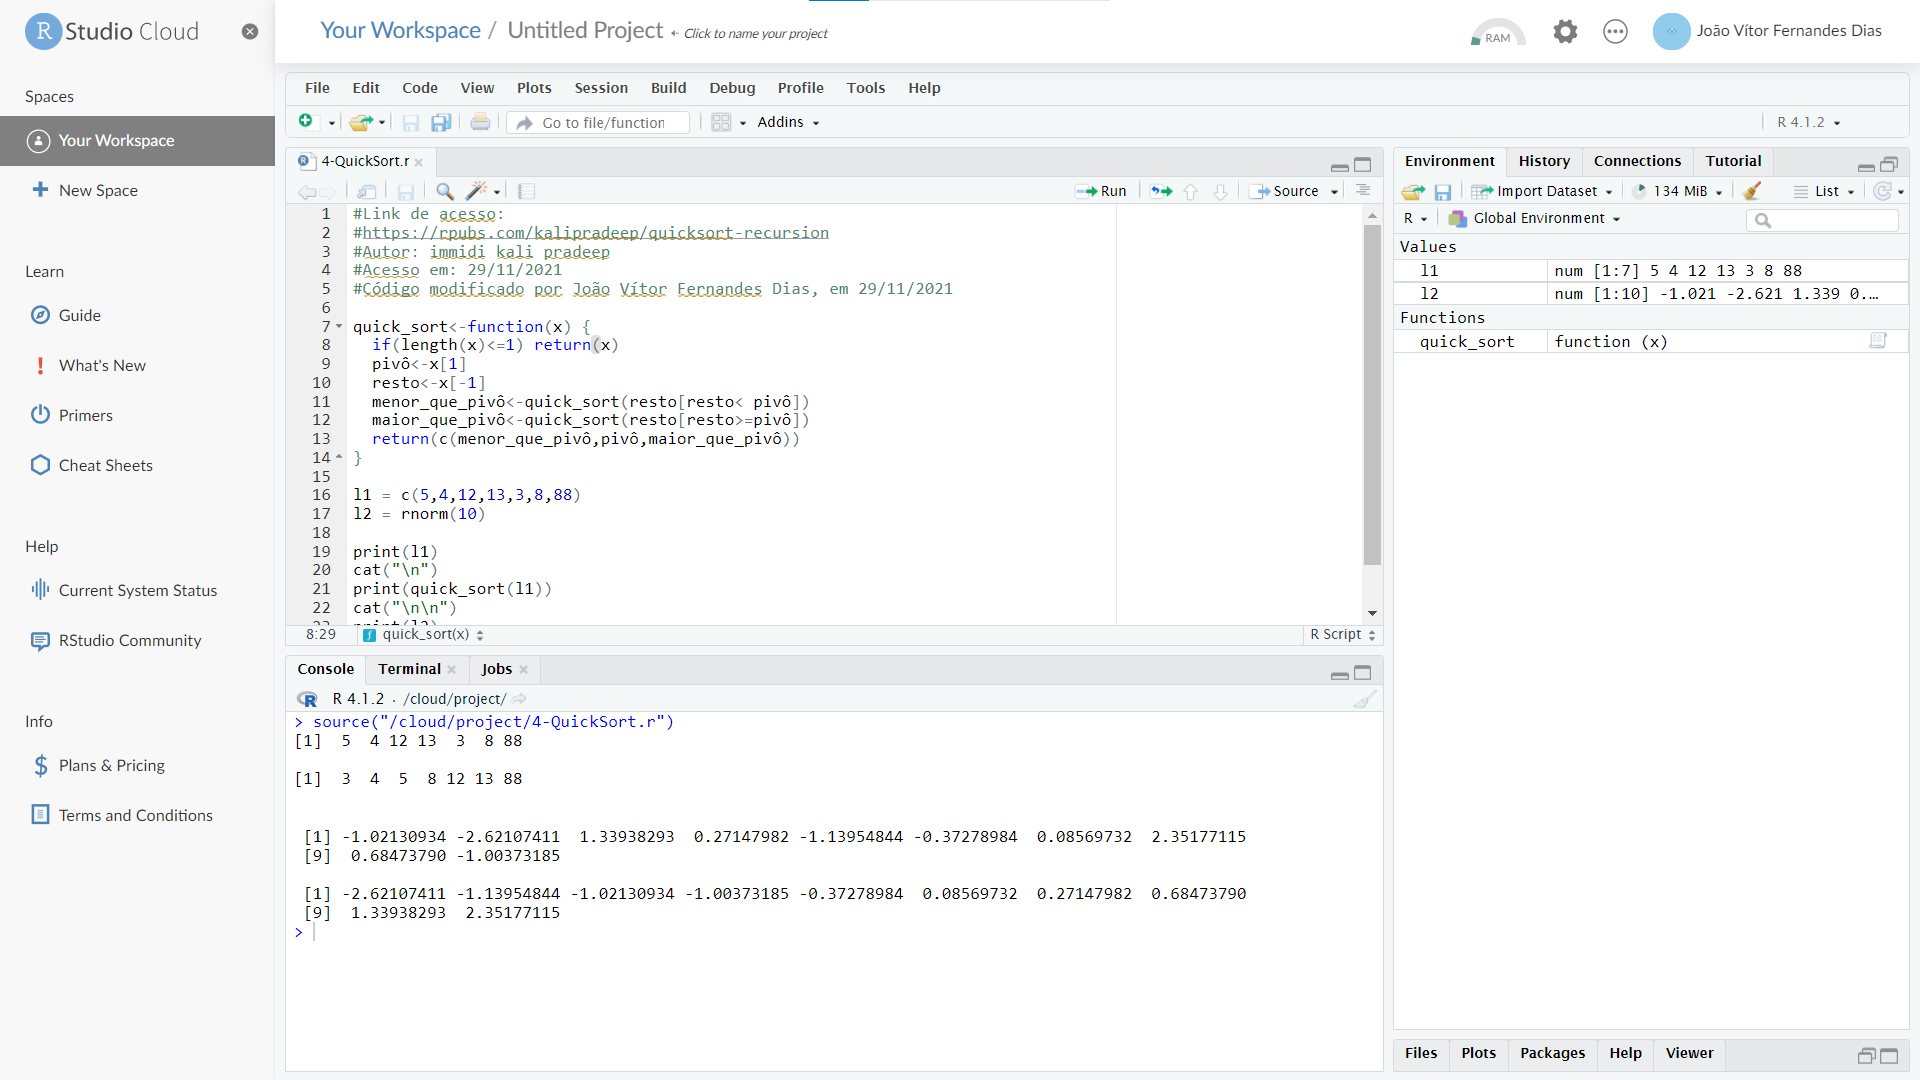
\includegraphics[width=16cm]{PicturesJoaoDias/Codigos/Codigo4_cloud.png}
        {\tiny \sf Fonte: autoria própria}
      \end{figure}
  	
  	\item \textbf{Links e referências bibliográficas das aplicações}
  	\\ \\
  	\textit{Link referente ao código:} 
  	\href{https://rpubs.com/kalipradeep/quicksort-recursion}{Quicksort Recursion}
  	
  	\textit{Desenvolvido por:} Immidi Kali Pradeep
  	
  	\textit{Acesso em:} 29/11/2021
  	
  \end{itemize}
	
  \section{Aplicações com Banco de Dados}
  \begin{itemize}
  	\item \textbf{Descrição}
  	
  	  O código abaixo apresenta duas formas de se lidar com um banco de dados. A primeira é mais simples e lida com dados inseridos manualmente em um data set. A segunda é mais avançada e próxima do uso geral de dados, que é utilizando um arquivo csv. No primeiro exemplo são listadas algumas pessoas e suas respectivas idades. No segundo exemplo é demonstrado o uso de dados estruturados referentes ao salário mínimo dos Estados Unidos entre os anos de 1938 e 2020.
  	
  	  Mais abaixo é mostrada a Figura \ref{Codigo_5} que representa a execução do código no ambiente de desenvolvimento RStudio.
  	  
  	\item \textbf{Código} 
  	
  	
  	\color{blue}
  	\verbatiminput{5-Database.r}
  	\color{black}
  	
  	\item \textbf{Aplicações com Banco de Dados no RStudio}
  	
	  	\begin{figure}[H]  \label{Codigo_5}
	  		\centering
	  		\caption{Gráfico resultante}
	  		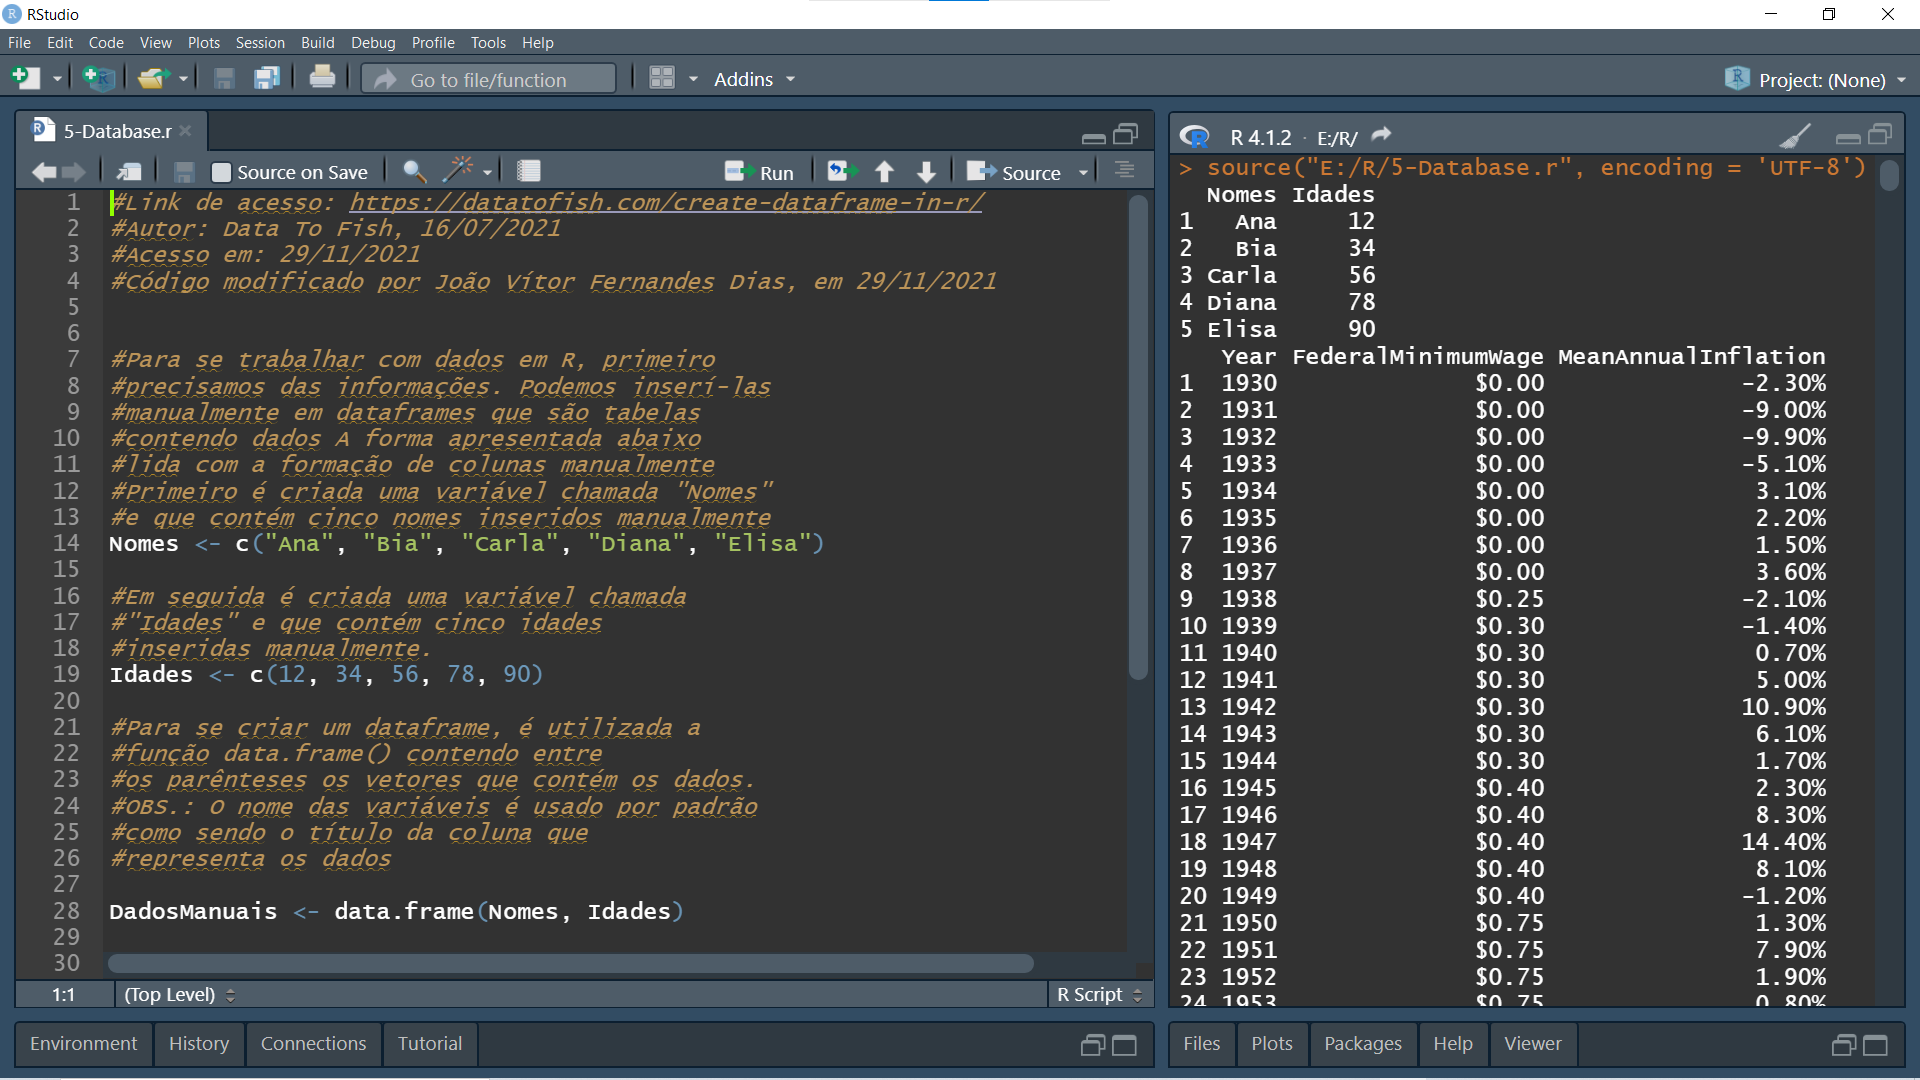
\includegraphics[width=16cm]{PicturesJoaoDias/Codigos/Codigo5.png}
	  		{\tiny \sf Fonte: autoria própria}
	  	\end{figure}
  	
  	\item \textbf{Links e referências bibliográficas das aplicações}
  	  \\ \\
  	  \textit{Link referente ao código:} 
  	  \href{https://datatofish.com/create-dataframe-in-r/}{Create  Dataframe in R}
  	  
  	  \textit{Desenvolvido por:} Data To Fish, 16/07/2021
  	  
  	  \textit{Acesso em:} 29/11/2021
  	  \\ \\
  	  \textit{Link referente ao arquivo CSV:}
  	  \href{https://www.kaggle.com/brandonconrady/us-minimum-wage-1938-2020}{US Minimum Wage 1938-2020}
  	  
  	  \textit{Desenvolvido por:} Brandon Conrady, 29/11/2021
  	  
  	  \textit{Acesso em:} 29/11/2021  	
  \end{itemize}